% FUNDAMENTACAO ------------------------------------------------------------------

\chapter{FUNDAMENTAÇÃO TEÓRICA}
\label{chap:fundamentacao}

\section{EMATER}
\label{subsec:emater}

O Instituto Paranaense de Assistência Técnica e Extensão Rural (EMATER) é uma autarquia vinculada à Secretaria de Estado da Agricultura e Abastecimento, que tem o papel de executar o serviço oficial de extensão rural do Estado \cite{ematerAE}.
A extensão rural tem como meta o progresso rural sustentável, por meio de assistência técnica focada na melhoria de renda dos agricultores em seus empreendimentos, qualidade de vida nas famílias no ambiente rural, avanço na competitividade e preservação dos recursos naturais e o meio ambiente.

A extensão rural oficial é disponibilizada em praticamente todo o estado. São 395 unidades que estendem aos agricultores de todos os municípios. Os beneficiários do processo de orientação são privilegiados os projetos que atendam as necessidades locais e regionais.

\section{PROGRAMA DE APOIO AO MANEJO E FERTILIDADE DO SOLO}
\label{subsec:pamfs}

O Programa de Apoio ao Manejo e Fertilidade do Solo, conhecido como Programa de Calcário, proporciona o uso de corretivos de solo aos agricultores familiares menos favorecidos, em busca do aumento de produtividade. O projeto ainda auxilia o pequeno agricultor na organização do processo de correção do solo, desde a identificação da necessidade de correção até a aplicação, incluindo o transporte e armazenagem \cite{ematerPAMFS}.

Entre os anos de 2013 e 2014, o programa beneficiou cerca de 35 mil produtores, aplicando aproximadamente 350 milhões de quilos de corretivos no solo, investindo entorno de 33,5 milhões de reais.

O Instituto Emater é responsável pela organização e aplicação do programa, divulgando, auxiliando na seleção dos favorecidos e definindo juntamente com os parceiros os planos de execução.

Além disso, o Instituto Emater também é responsável pela elaboração de projetos técnicos, pela orientação aos agricultores na coleta de amostras de solo e na recomendação do uso de corretivos agrícolas.

\section{CORREÇÃO E EQUILÍBRIO DO SOLO}
\label{subsec:correcaodosolo}

A terra é o elemento central da agricultura e precisa de um bom manejo para que haja uma boa safra. Mesmo que seja feita uma boa adubação, algumas plantas, como a soja e o milho, não se desenvolvem bem em um pH ácido \cite{de2003sugestao}, pois a disponibilidade de nutrientes está diretamente relacionada à acidez do solo. Por isso, a correção do solo pode ser determinante para uma colheita farta ou mediana, contribuindo para o aumento da renda e, consequentemente, da qualidade de vida do produtor rural.

Diversos fatores contribuem para o desempenho do terreno como a compactação do solo e a pluviosidade, mas a acidez é o principal deles. Devido à fatores geológicos, o Brasil tende a possuir uma grande concentração de íons de hidrogênio e alumínio \cite{bookfa2215c6}. Dessa forma, nutrientes essenciais como nitrogênio, fósforo e potássio têm sua disponibilidade comprometida, afetando o crescimento do vegetal.

O alumínio e manganês, quando disponibilizados em excesso, são tóxicos para a plantação \cite{malavolta1980effects}. Ao contrário dos nutrientes supracitados, esses aumentam quando o pH diminui. A presença desses elementos prejudicam o desenvolvimento do sistema radicular, muitas vezes causando o tombamento da planta, prejudicando a absorção de nutrientes e a produtividade da cultura.

Para aumentar o pH, deve-se realizar a calagem , que é a aplicação de calcário no terreno \cite{rossetto}. A qualidade e rapidez de incorporação e a dose recomendada do calcário está diretamente relacionada ao Poder Real de Neutralização Total (PRNT) do corretivo.

\section{PLANILHA DE CORREÇÃO DE SOLOS}
\label{subsec:planilha}

Atualmente a Emater utiliza uma planilha eletrônica desenvolvida para o Microsoft Excel por Pedro Cecere Filho e Fabianderson J. B. de Souza e contou com o apoio de Nelson Hargerm, Celso D. Seratto e Adilson O. Junior, para a realização dos cálculos de correção e equilíbrio do solo.

O objetivo dessa planilha é gerar um relatório de recomendações para a correção do solo de um determinado talhão com base no laudo técnico do solo, na cultura desejada, na produtividade desejada. Além disso a planilha também fornece a quantidade e o valor aproximado de cada corretivo agrícola que o produtor deverá adquirir para suprir as necessidades da planta. 

A planilha é composta por 5 pastas de trabalho que serão enumeradas e descritas nas subseções abaixo.

\subsection{Pasta de Trabalho: Ajuda}
\label{subsec:pastaajuda}

Nessa pasta estão descritas algumas instruções para o correto uso da planilha, bem como os créditos aos participantes no desenvolvimento, o telefone de contato do técnico responsável para esclarecimento de dúvidas e a data da última atualização, conforme é exibido na \autoref{fig:pastaajuda}.

\begin{figure}[H]
    \centering
    \caption{Pasta de Trabalho: Ajuda}
    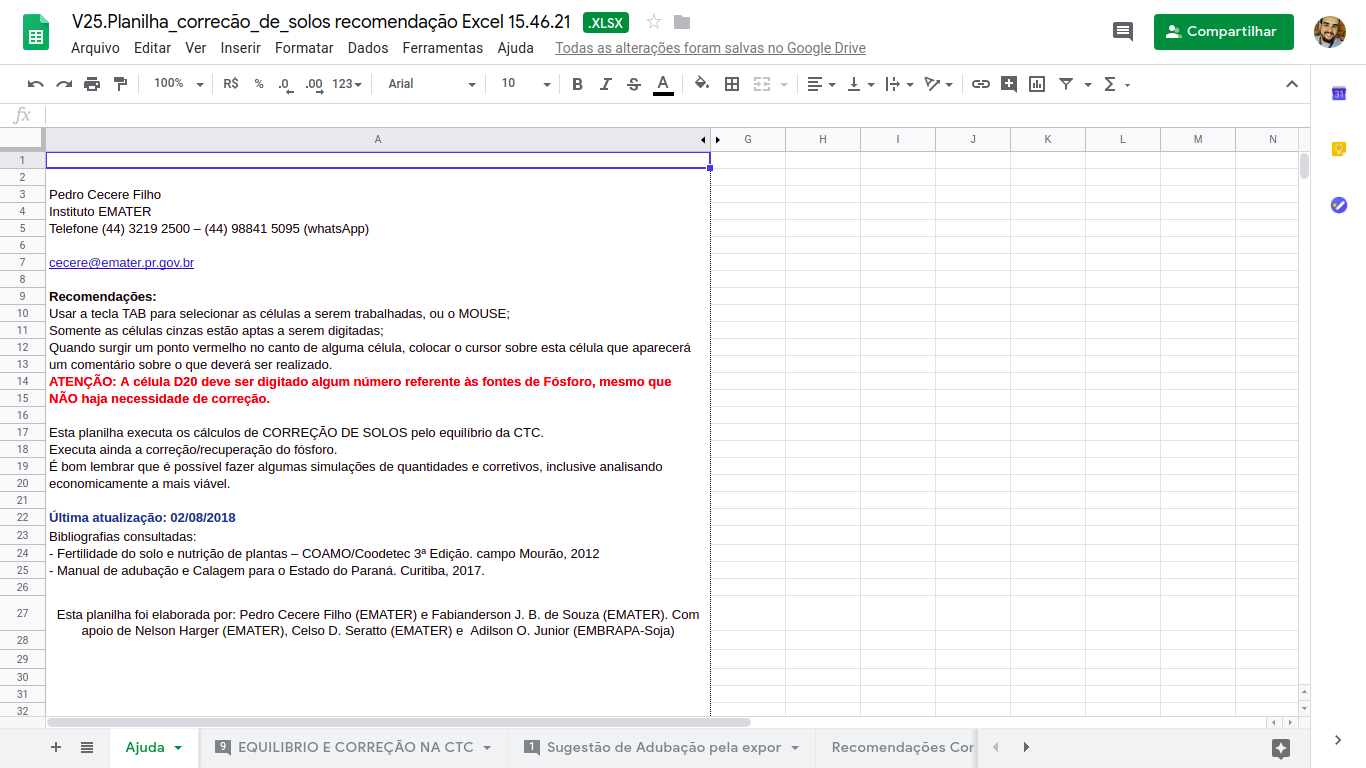
\includegraphics[width=13cm]{dados/figuras/planilha/tab-ajuda.png}
    \label{fig:pastaajuda}
    \fonte{Planilha de Correção do Solo}
\end{figure}

\subsection{Pasta de Trabalho: Equilíbrio e Correção na CTC}
\label{subsec:pastaequilibriocorrecaoctc}

Esta é a pasta de trabalho na qual o técnico informa os dados acerca do local a ser corrigido. Para facilitar o entendimento, o formulário será dividido em 5 seções que estão descritas nas próximas subseções. Deve-se considerar que os campos com o fundo em cinza são entradas do usuário.

O objetivo dessa pasta é fornecer uma visão geral dos três momentos da área analisada: como ela está atualmente, como ela deverá estar após as correções e como seria no caso ideal. O valor ideal depende da cultura considerada para o talhão. A planilha apresentada só considera as possibilidades de cultivo de soja e milho nas áreas corrigidas.

É importante salientar que existem diferentes métodos de avaliação para a calagem do solo. Porém, a planilha aborda apenas o método de saturação por bases. Este é o método é praticado apenas nas regiões de SP e PR \cite{rossetto}.

\subsubsection{Identificação da Propriedade}
\label{subsubsec:identificacao}
Esta seção é responsável pela entrada de dados referentes ao local de coleta da amostra de terra, denominado talhão, enviada para a análise em laboratório. Para identificação do talhão a planilha solicita ao usuário as seguintes entradas: do nome do proprietário, a data do cálculo, o município e lote onde esta está situada, a área total em hectares, a identificação do talhão, a área do talhão em hectares e a matrícula do lote além do nome do técnico da Emater responsável por essa região e o tipo de plantio aplicado, que pode ser o convencional ou direto.

\begin{figure}[H]
    \centering
    \caption{Identificação do Talhão}
    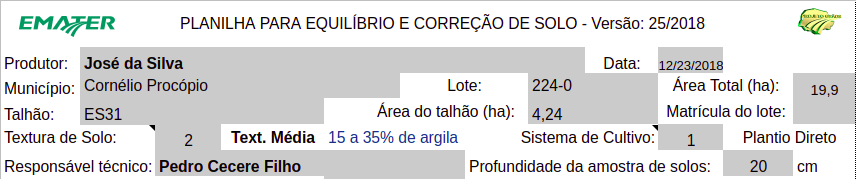
\includegraphics[width=13cm]{dados/figuras/planilha/corr_info_propriedade.png}
    \label{fig:identificacaotalhao}
    \fonte{Planilha de Correção do Solo}
\end{figure}

Outros dados relevantes para o cálculo da correção do solo como profundidade da amostra em centímetros e textura do solo, que pode ser argilosa ou textura média dependendo da proporção de argila, também são colhidos nessa seção.

\subsubsection{Resultado da Análise Química do Solo}
\label{subsubsec:analisequimica}

O laudo técnico do solo é emitido por um laboratório de análise do solo e possui um número de identificação. Ele apresenta as características físicas e químicas do solo. Dentre as características físicas, a textura do solo é indispensável para o cálculo da correção. Outras informações como profundidade da amostra coletada e o sistema de cultivo também são importantes.

A planilha considera apenas duas variações de textura do solo: o argiloso e o de textura média. O solo argiloso é aquele que possui argila em pelo menos 35\% de sua composição, enquanto o de textura média varia entre 15\% e 35\%.

Os teores de nutrientes do solo também são provenientes do laudo técnico, que pode ser observado no \autoref{chap:laudodosolo}. Os nutrientes considerados na planilha são o fósforo (P), o potássio (K), o Cálcio (Ca), o Magnésio (Mg), o Enxofre (S), o Alumínio (Al) e a acidez potencial (soma do Hidrogênio e o Alumínio). Os valores de P são informados em \(mg/dm^3\), enquanto o K, Ca, Mg, S, H e Al são fornecidos em \(cmol/dm^3\).

\begin{figure}[H]
    \centering
    \caption{Laudo Técnico do Solo}
    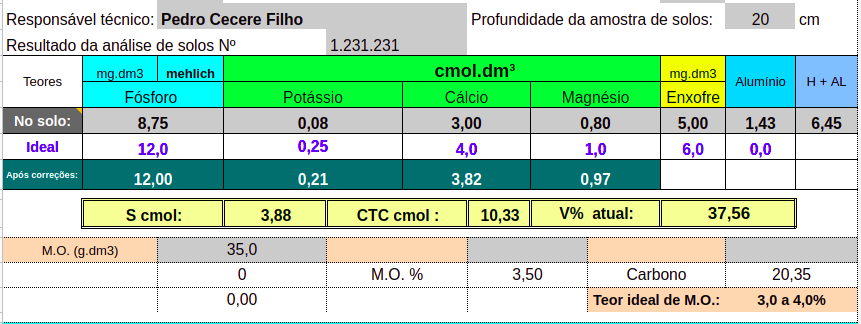
\includegraphics[width=13cm]{./dados/figuras/planilha/corr_analise_quimica.png}
    \label{fig:analisequimicatabela}
    \fonte{Planilha de Correção do Solo}
\end{figure}

A planilha calcula e exibe dinamicamente os valores ideais dos nutrientes de acordo com a textura do solo e também qual será o teor de cada substância após a aplicação das correções.

Ainda na seção de análise do solo, o técnico informa o teor de matéria orgânica presente no solo. Como a unidade de medida depende do laboratório que emitiu o laudo, esse valor pode ser informado em \(g/dm^3\), percentual (\%) ou em carbono.

\subsubsection{Correção/Recuperação do Fósforo}
\label{subsubsec:corrrecfosforo}

Na seção de correção/recuperação do fósforo, o usuário deve fornecer informações para o cálculo de equilíbrio referente ao fósforo. O técnico deve informar qual é o teor desejado de fósforo em \(mg/dm^3\), qual será o corretivo será aplicado, a eficiência do fósforo do corretivo em percentual e o valor em R\$/ton da fonte de fósforo.

\begin{figure}[H]
    \centering
    \caption{Correção/Recuperação do Fósforo}
    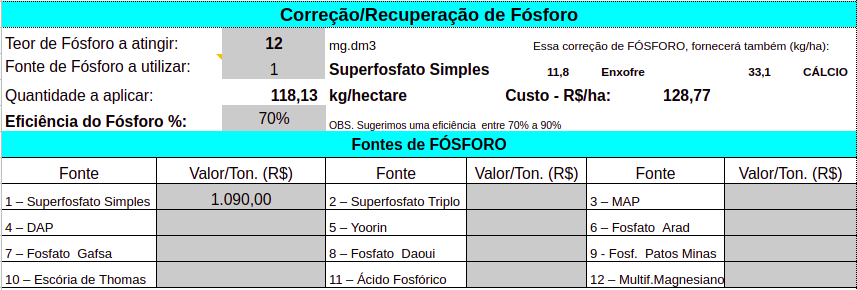
\includegraphics[width=13cm]{./dados/figuras/planilha/corr_rec_fosforo.png}
    \label{fig:correcaorecfosforo}
    \fonte{Planilha correção de solos}
\end{figure}

Após o preenchimento dos campos, o sistema consegue calcular ativamente a quantidade a ser aplicada e o custo em R\$/ha do fertilizante, além da quantidade em quilos de outros nutrientes que esta aplicação incrementará ao solo.

\subsubsection{Correção/Recuperação do Potássio}
\label{subsubsec:corrrecpotassio}

Nesta seção, a planilha exibe ao técnico o percentual da participação do potássio atualmente na CTC, solicita o percentual desejado, exibe o percentual ideal, exibe o percentual que esperado após as correções, além de solicitar a fonte de potássio e o custo em R\$/ton desse corretivo.

\begin{figure}[H]
    \centering
    \caption{Correção/Recuperação do potássio}
    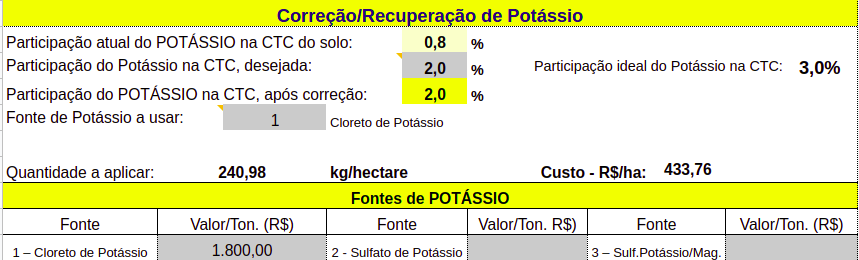
\includegraphics[width=13cm]{./dados/figuras/planilha/corr_rec_potassio.png}
    \label{fig:correcaorecpotassio}
    \fonte{Planilha correção de solos}
\end{figure}

Após o preenchimento dos campos em cinza, o sistema calcula e exibe dinamicamente a quantidade a ser aplicada e o custo em R\$/ha do fertilizante, além da quantidade em quilos de outros nutrientes que este corretivo fornecerá.

\subsubsection{Correção/Recuperação do Cálcio e Magnésio}
\label{subsubsec:corrreccalciomagnesio}

Nessa última seção de correção, a planilha recebe as entradas referentes à correção/recuperação do cálcio e magnésio. Nessa parte a planilha exibe o percentual de cálcio e magnésio presentes atualmente e o percentual ideal desses nutrientes na CTC de acordo com a textura de solo selecionada. Espera-se como entrada o percentual de cálcio desejado na CTC, a fonte de cálcio que será utilizada na correção e o custo em R\$/ton, além do PRNT e o teor de CaO da fonte de corretivo.

\begin{figure}[H]
    \centering
    \caption{Correção/Recuperação do Cálcio e Magnésio}
    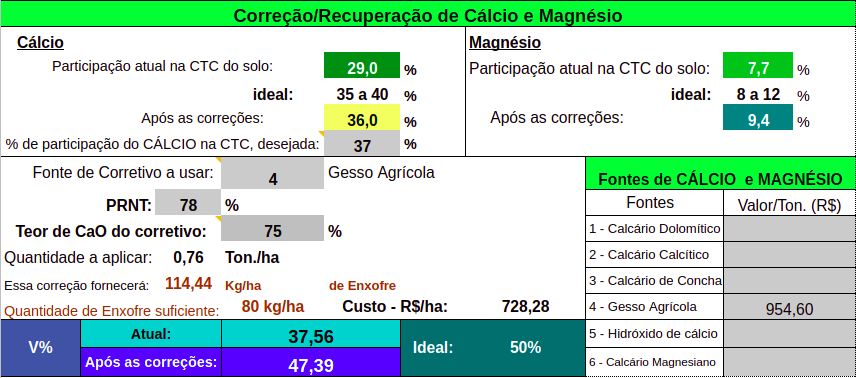
\includegraphics[width=13cm]{./dados/figuras/planilha/corr_rec_calcio_magnesio.png}
    \label{fig:correcaoreccalciomagnesio}
    \fonte{Planilha correção de solos}
\end{figure}

Com essas informações preenchidas, o sistema é capaz de calcular dinamicamente a quantidade da fonte de corretivo necessária para a correção em ton/ha, o custo em R\$/ha e a quantidade de outros nutrientes como o enxofre e que serão fornecidos à mistura. Além disso, também será possível informar o teor de Magnésio no solo após as correções.

O cálculo da necessidade de calagem se dá pela seguinte fórmula:

\[ NC
  = \dfrac{(V2 - V1) * CTC}{10 * PRNT}
\]

Sendo que:
\begin{itemize}
    \item NC: Necessidade de calagem
    \item V2: Saturação de bases desejada
    \item V1: Saturação de bases encontrada no solo
    \item CTC é a capacidade de troca de cátions, ou \(Ca + Mg + K + Na + (H + Al)\)
    \item PRNT: Poder Relativo de Neutralização Total
\end{itemize}

\subsubsection{Saturação por Bases}
\label{subsubsec:resultadosaturacao}

Nas últimas linhas da planilha desta pasta de trabalho são calculados os valores da saturação por bases (V\%) obtidos por meio dos cálculos com as informações fornecidas pelo usuário, como pode ser observado na \autoref{fig:saturacaoporbase}.

\begin{figure}[H]
    \centering
    \caption{Saturação de Base}
    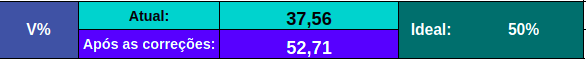
\includegraphics[width=13cm]{./dados/figuras/planilha/corr_saturacao.png}
    \label{fig:saturacaoporbase}
    \fonte{Planilha correção de solos}
\end{figure}

O valor de V\% representa o equilíbrio das bases na CTC. No caso do milho e da soja, para o melhor desenvolvimento desses vegetais, recomenda-se a saturação em 50\%.

\subsection{Pasta de Trabalho: Sugestão de adubação pela exportação}
\label{subsec:sugestaoadubacao}

Essa pasta de trabalho tem como objetivo gerar um plano de correção do solo baseado nas informações processadas na \autoref{subsec:pastaequilibriocorrecaoctc}. O usuário deve informar qual é a cultura que será destinada aquele talhão e a produtividade esperada em sacas/alqueire, além do percentual de eficiência fósforo do corretivo.

\subsection{Pasta de Trabalho: Memória de Cálculo}
\label{subsec:memoriadecalculo}

Essa pasta de trabalho armazena as fórmulas para a correção do fósforo, potássio, cálcio e magnésio e está dividida em 3 seções.

\subsection{Pasta de Trabalho: Recomendações Correção e Adubação}
\label{subsec:recomendacoes}

Essa pasta de trabalho é responsável pela geração do documento final de orientação de correção. Nela o técnico descreve como deverá ser corrigido cada um dos indicadores, indicando a quantidade e o valor em R\$/tonelada de cada corretivo.

No rodapé são dispostos dois campos para que o proprietário e o técnico façam a assinatura da recomendação.
